\section{Introduction to machine learning}
\only<presentation>{
  \begin{frame}
    \tableofcontents[ 
    currentsection, 
    hideothersubsections, 
    sectionstyle=show/shaded
    ] 
  \end{frame}
}


\only<article>{
  What are the central problems in machine learning?

  Problems in machine learning are similar to problems in science.
  Scientists must plan experiments intelligently and collect data.
  The must be able to use the data to verify a different hypothesis.
  More generally, they must be able to make decisions under
  uncertainty (Without uncertainty, there would be no need to gather more data).
  Similar problems appear in more mundane tasks, like learning to drive a car.
}
\only<presentation>{
  \begin{frame}
    \frametitle{Scientific applications}
    \centering
    \begin{columns}
      \begin{column}{0.5\textwidth}
        \centering
        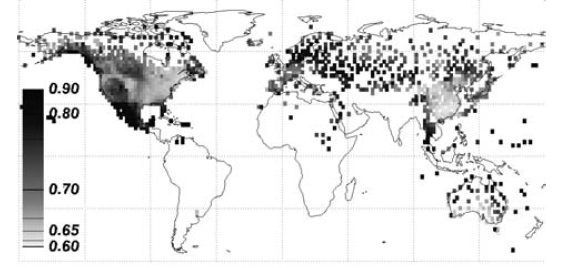
\includegraphics[width=0.8\columnwidth]{../figures/climate.jpg}\\
        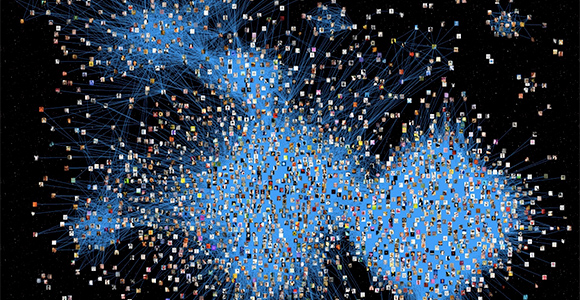
\includegraphics[width=\columnwidth]{../figures/networks-2.jpg}
      \end{column}
      \begin{column}{0.5\textwidth}
        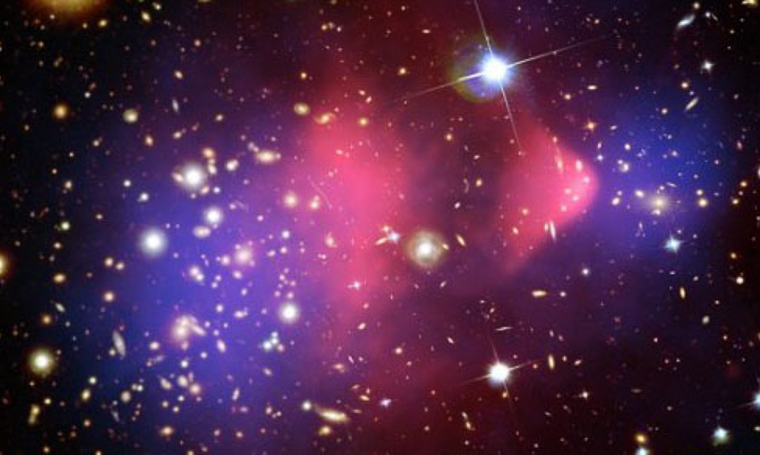
\includegraphics[width=\columnwidth]{../figures/dark_matter.jpg}
        \\
        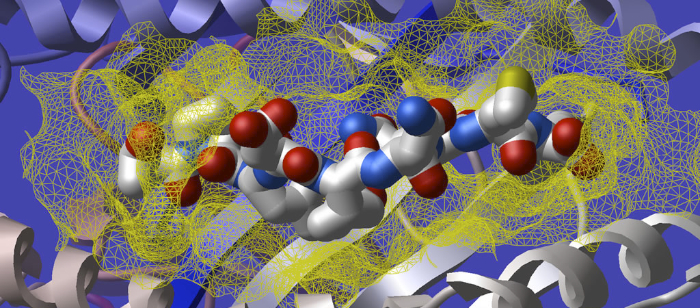
\includegraphics[width=\columnwidth]{../figures/protein.jpg}
      \end{column}
    \end{columns}
    \only<2>{
      \begin{tikzpicture}[remember picture,overlay]
        \draw[fill=black,opacity=0.75] 
        (current page.north east) rectangle (current page.south west);
        \node at (current page.center) {
          {\Huge \alert{Interpretability, Reproducibility}}
        };
      \end{tikzpicture}}
  \end{frame}
}

\only<article>{
  For that reason, science is a very natural application area for
  machine learning.  We can model the effects of climate change and
  how to mitigate it; discover structure in social networks; map
  the existence of dark matter in the universe by intelligently
  shifting through weak gravitational lens data, and not only study
  the mechanisms of protein folding, but discover methods to
  synthesize new drugs.

  We must be careful, however. In many cases we need to be able to
  interpret what our model tells us. We also must make sure that
  the any results we obtain are reproducible. This is something
  that we shall emphasize in this course.
}

\only<presentation>{
  \begin{frame}
    \frametitle{Pervasive ``intelligent'' systems}
    \begin{columns}
      \begin{column}{0.3\textwidth}
        \centering
        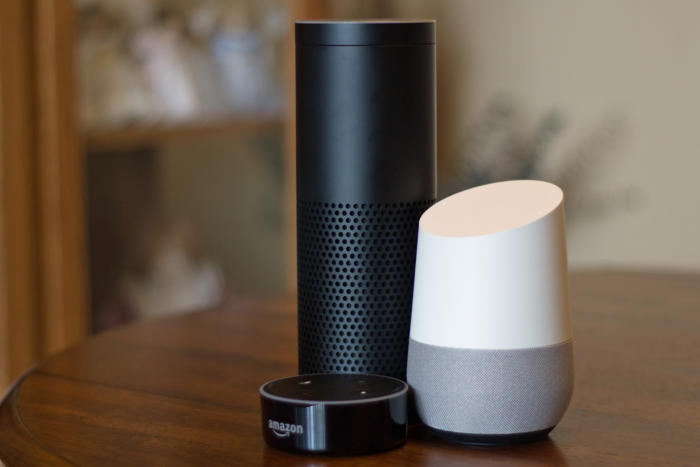
\includegraphics[width=\textwidth]{../figures/echo-home.jpg}
        \\
        Home assistants

        \vspace{\fill}

        \bigskip

        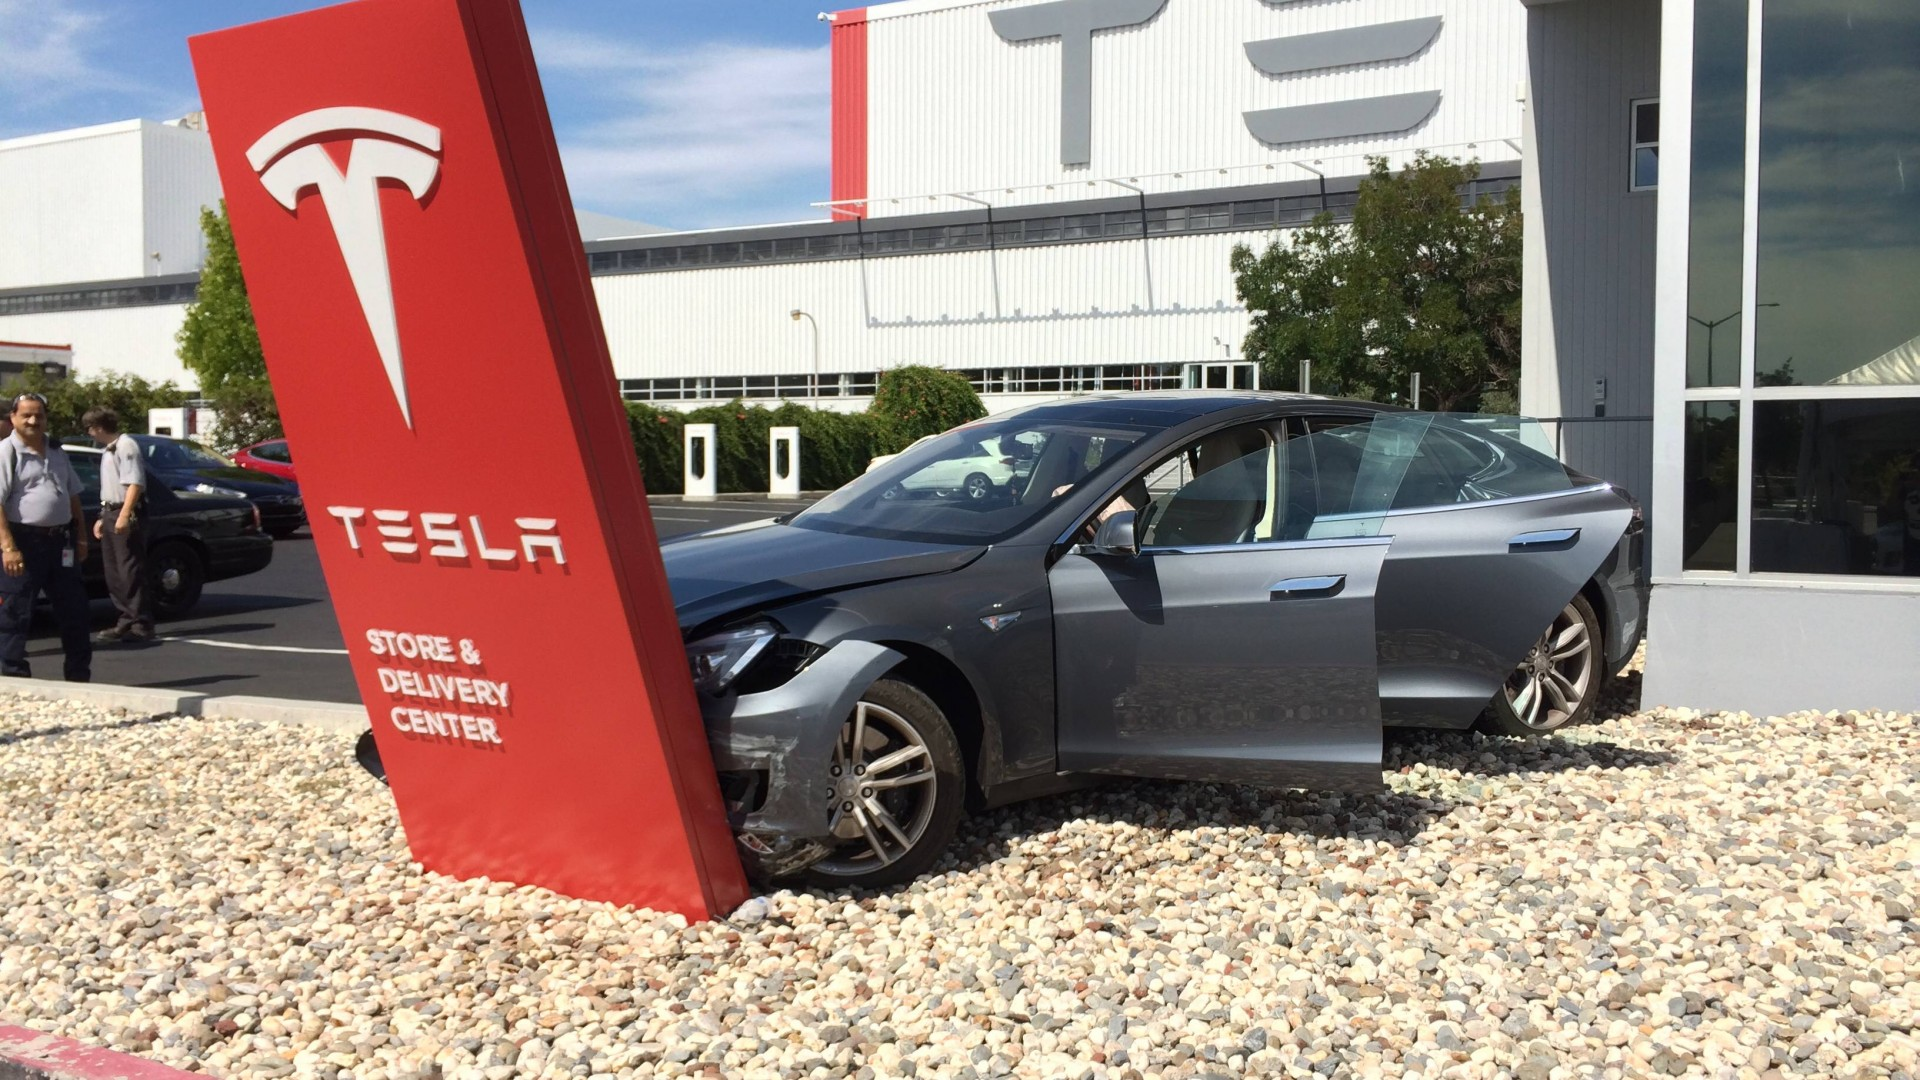
\includegraphics[width=\textwidth]{../figures/tesla.jpg}
        \\
        Autonomous vehicles
      \end{column}
      \begin{column}{0.3\textwidth}
        \centering 
        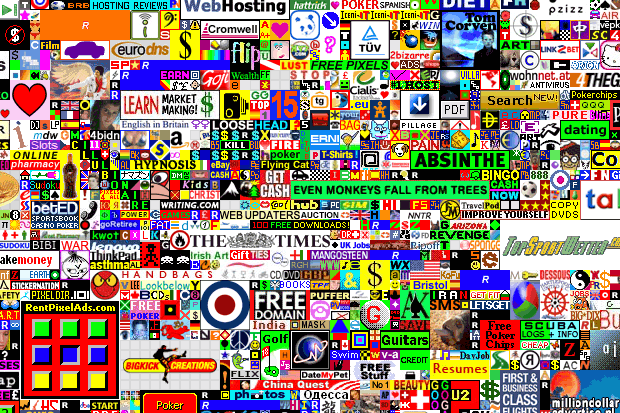
\includegraphics[width=\textwidth]{../figures/web-ads.png}
        \\
        Web advertising

        \vspace{\fill}

        \bigskip

        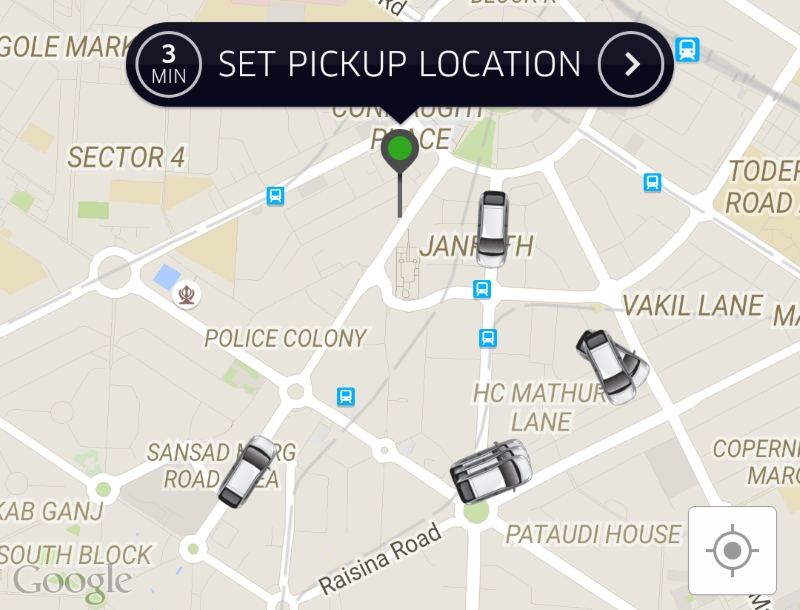
\includegraphics[width=\textwidth]{../figures/uber-here-maps.jpg}
        \\
        Ridesharing
      \end{column}
      \begin{column}{0.3\textwidth}
        \centering 
        \\
        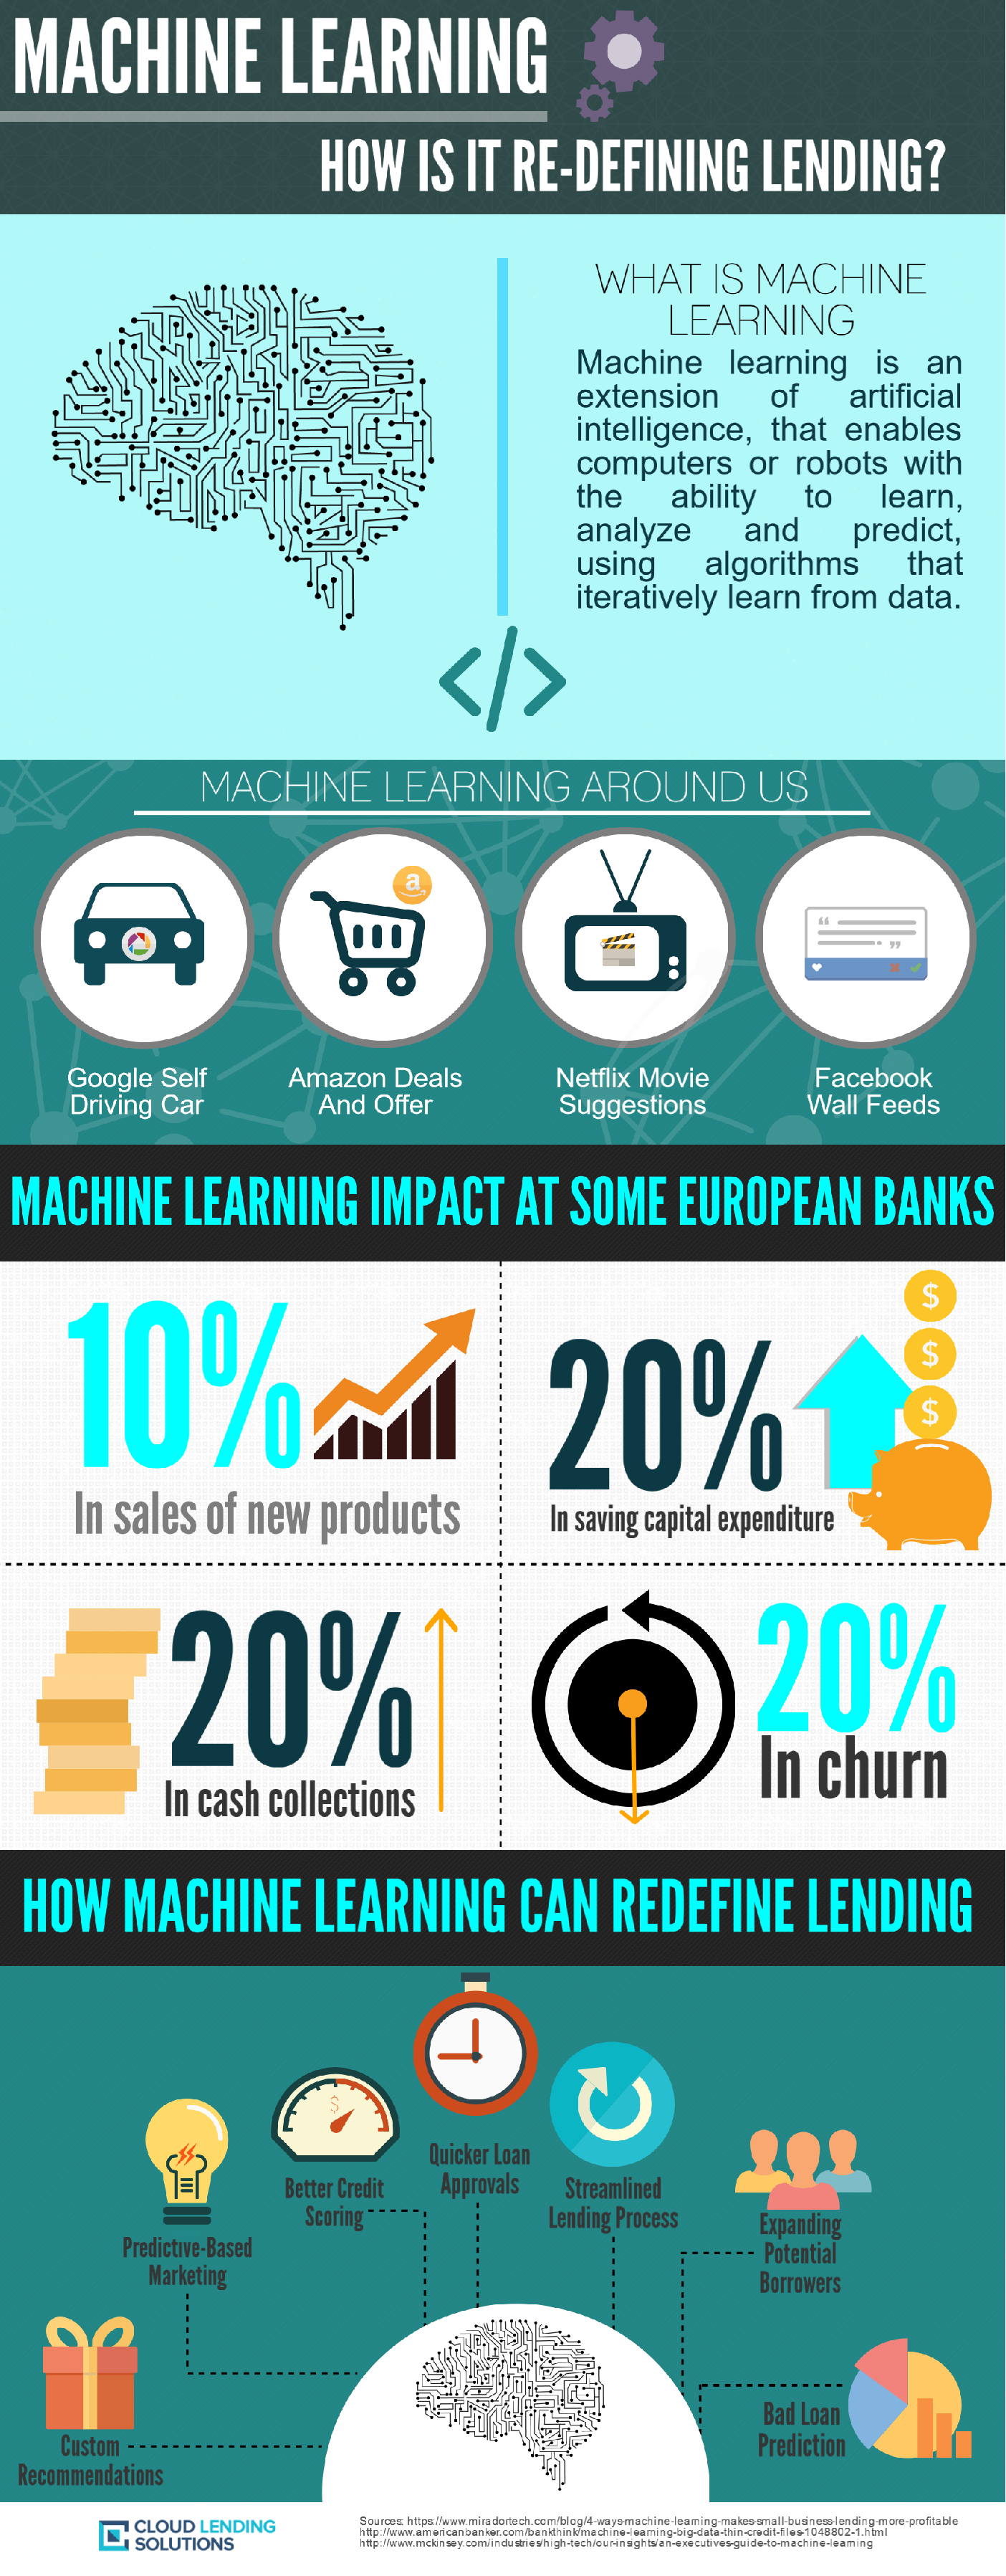
\includegraphics[width=\textwidth,clip = true, trim=0 0 0 42.5cm]{../figures/lending.pdf}
        \\
        Lending

        \vspace{\fill}

        \bigskip

        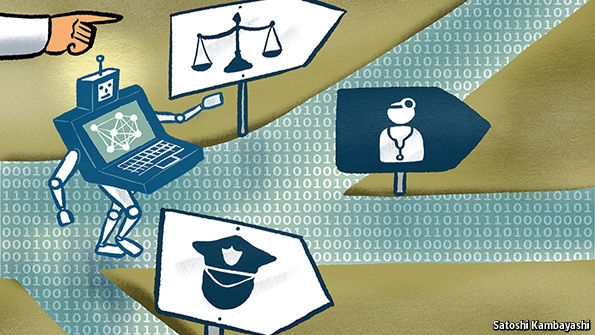
\includegraphics[width=\textwidth]{../figures/algorithms-public.jpg}
        \\
        Public policy
      \end{column}
    \end{columns}
    \only<2>{
      \begin{tikzpicture}[remember picture,overlay]
        \draw[fill=black,opacity=0.75] 
        (current page.north east) rectangle (current page.south west);
        \node at (current page.center) {
          {\Huge \alert{Privacy, Fairness, Safety}}
        };
      \end{tikzpicture}}
  \end{frame}
}

\only<article>{
  While machine learning models in science are typically carefully
  handcrafted by scientists and experts in machine learning and
  statistics, this is not typically the case in everyday
  applications. Nevertheless, well-known or home-grown machine
  learning models are being deployed across the application
  spectrum. This involve home assistants that try and get you want,
  web advertising, which tries to find new things for you to want,
  lending, which tries to optimally lend you money so that you buy
  what you didn't need before. We also have autonomous vehicles,
  which take you were you want to go, and ridesharing services,
  which do the same thing, but use humans instead. Finally, there
  are many applications in public policy, such as crime prevention,
  justice, and disease control which use machine learning.  In all
  those cases, we have to worry about a great many things that are
  outside the scope of the machine learning problems itself. These
  are (a) privacy: you don't want your data used in ways that you have
  not consented to (b) fairness: you don't want minorities to be
  disadvantaged and (c) safety: you don't want your car to crash.
}

\subsection{Data analysis,  learning and planning}

\only<article>{
  To make the above more concrete, let's have a look at a number of problems in machine learning. These involve learning from and analysing data, including inferring decision rules, and constructing complex plans using the evidence gleaned from the data. Machine learning problems are commonly separated in three different types: supervised, unsupervised and reinforcement learning. Typical supervised learning problems include classification and regression, while unsupervised problems include compression, clustering and topic modelling. Reinforcement learning, on the other hand, is concerned with artificially intelligent agents more generally, with examples including game playing and adaptive control. Their main differences are two. Firstly, the \emph{type} of feedback we have about learning performance. Secondly, and perhaps more importantly, whether or not the problem involves \emph{active data collection}. In this course, we will try and take a global view of these problems in the context of decision theory.
}

\only<presentation>{
  \begin{frame}
    \centering
    \Huge{What can machine learning do?}
  \end{frame}
}
\begin{frame}
  \frametitle{Can machines learn from data?}
  \begin{center}
    \only<1>{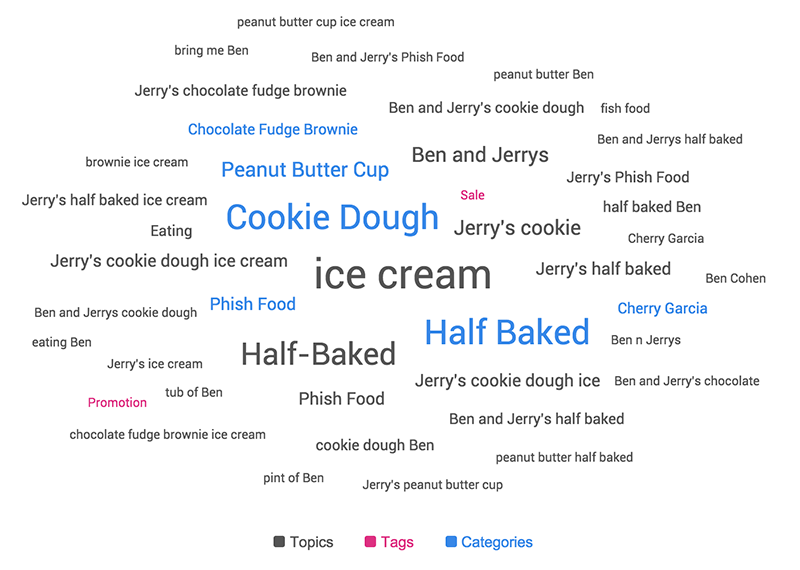
\includegraphics[width=0.8\textwidth]{../figures/text-cloud}
      \\

      {\large An unsupervised learning problem: topic modelling}
    }
    \only<2>{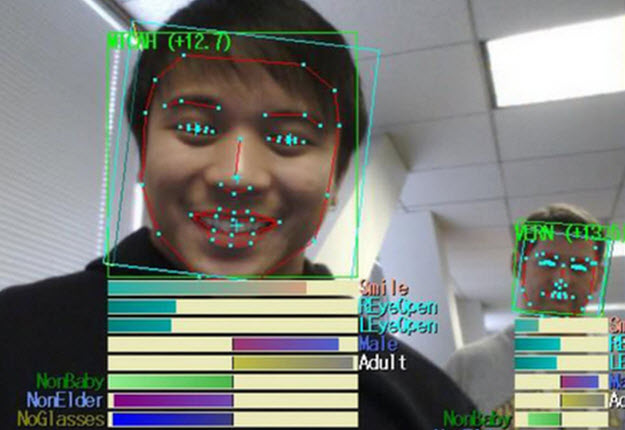
\includegraphics[width=0.8\textwidth]{../figures/Face-Recognition}
      \\

      {\large A supervised learning problem: object recognition}
    }
  \end{center}
\end{frame}


\only<article>{
  You can use machine learning just to analyse, or find structure in
  the data. This is generally called unsupervised learning. One such
  example is topic modelling, where you let the algorithm find topics
  from a corpus of text.  These days machines are used to learn from
  in many applications.  These include speech recognition, facial
  authentication, weather prediction, etc. In general, in these
  problems we are given a \emph{labelled} dataset with, say, example
  images from each class. Unfortunately this does not scale very
  well, because obtaining labels is expensive.

  This is partially how science works, because what we need to do
  is to find a general rule of nature from data. Starting from some
  hypothesis and some data, we reach a conclusion. However, many
  times we may need to actively experiment to obtain more data,
  perhaps because we found that our model is wrong.
}



\begin{frame}
  \frametitle{Can machines learn from their mistakes?}
  \begin{center}
    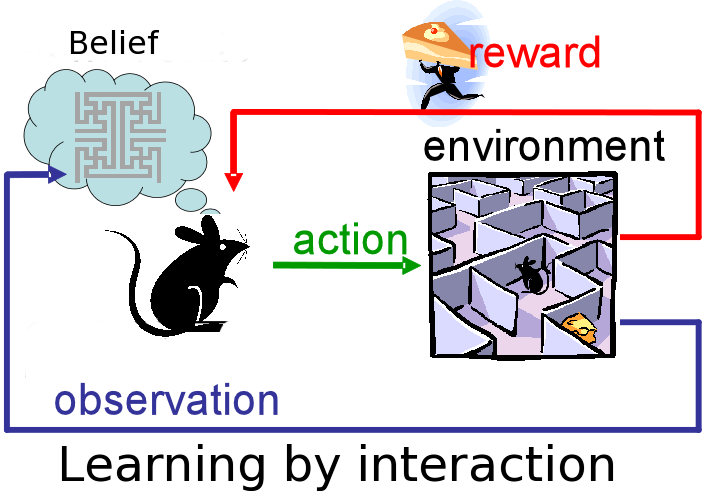
\includegraphics[width=0.7\textwidth]{../figures/rl_interaction}
  \end{center}
  \begin{block}{Reinforcement learning}
    Take actions $a_1, \ldots, a_t$, so as to maximise utility
    $U = \sum_{t=1}^T r_t$
  \end{block}
\end{frame}


\only<article>{
  So, what happens when we make a mistake? Can we somehow recognise
  it? Humans and other animals can actually learn from their
  mistakes. Consider the proverbial rat in the maze. At some
  intervals, the experimenter places some cheese in there, and the
  rat must do a series of actions to obtain it, such as navigating
  the maze and pulling some levers. It doesn't know how to get to
  the cheese easily, but it slowly learns the layout of the maze
  through observation, and in the end, through trial-and-error it
  is able to get to the cheese very efficiently.

  We can formalise this as a reinforcement learning problem, where
  the rat takes a series of actions; at each step it also obtains a
  reward, let's say equal to 0 when it has no cheese, and 1 when it
  eats cheese. Then we can declare that the rat's utility is the sum
  of all rewards over time, i.e. the total amount of cheese it can
  eat before it dies. The rat needs to explore the environment in order to be able to
  get to the cheese. 

  An example in robotics is trying to teach a
  robot to flip pancakes. One easy thing we can try is to show the robot
  how to do it, and then let it just copy the demonstrated
  movement. However, this doesn't work! The robot needs to explore
  variations of the movement, until it manages to successfully flip
  pancakes. Again, we can formulate this as a reinforcement learning
  problem, with a reward that is high whenever the pancake's position is
  flipped, and on the pan; and low everywhere else. Then the robot can
  learn to perform this behaviour through trial and error. It's
  important to note that in this example, merely demonstration is not
  enough. Neither is reinforcement learning enough. The same thing is
  true for the recent success of AlphaGo in beating a master human:
  apart from planning, they used both demonstration data and self-play,
  so that it could learn through trial and error.  }

\begin{frame}
  \frametitle{Can machines make complex plans?}
  \begin{center}
    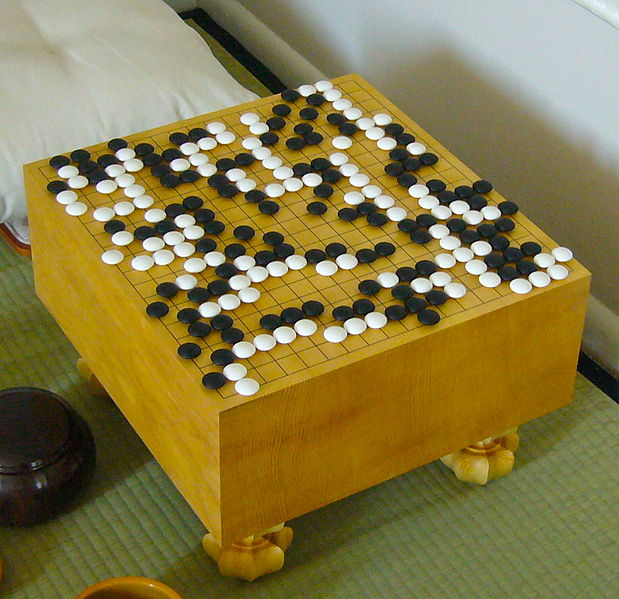
\includegraphics[width=0.8\textwidth]{../figures/619px-FloorGoban}
  \end{center}
\end{frame}


\only<article>{
  I suppose the first question is whether machines can plan
  ahead. Indeed, even for large problems, such as Go, machines can
  now perform at least as well as top-rated humans. How is this
  achieved?
}

\begin{frame}
  \frametitle{Machines can make complex plans!}
  \begin{center}
    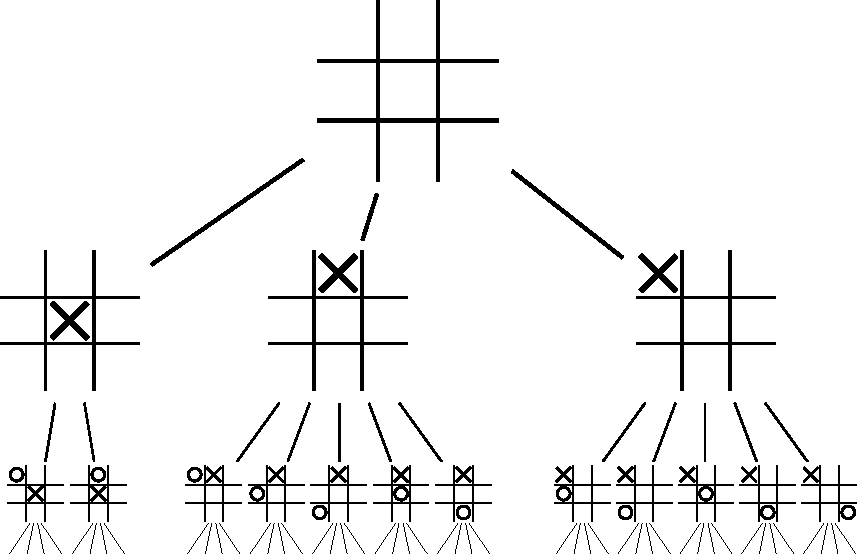
\includegraphics[width=0.8\textwidth]{../figures/Tic-tac-toe-game-tree}
  \end{center}
\end{frame}


\only<article>{
  The basic construction is the planning tree. This is an enumeration
  of all possible future events. If a complete enumeration is
  impossible, a partial tree is constructed. However this requires
  evaluating non-terminal game positions. In the old times, this was
  done with heuristics, but now this is data-driven, both through the
  use of expert databases, and through self-play and reinforcement
  learning.
}


\subsection{Experiment design}

\only<presentation>{
  \begin{frame}
    \centering
    \Huge{The scientific process as machine learning}
  \end{frame}
  \begin{frame}
    \centering
    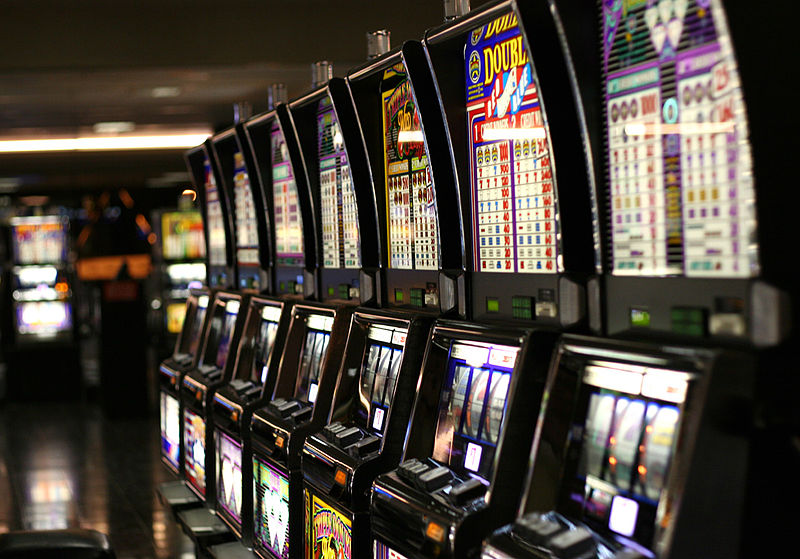
\includegraphics[width=\textwidth]{../figures/Las_Vegas_slot_machines}
  \end{frame}
}


\only<article>{
  An example that typifies trial and error learning are bandit
  problems. Imagine that you are in a Casino and you wish to
  maximise the amount of money you make during the night. There are
  a lot of machines to play. If you knew which one was the best,
  then you'd just play it all night long. However, you must also
  spend time trying out different machines, in order to get an
  estimate of how much money each one gives out. The trade off
  between trying out different machines and playing the one you
  currently think is best is called the exploration-exploitation
  trade-off and it appears in many problems of experiment design for
  science.
}


\begin{frame}
  \frametitle{Adam, the robot scientist}
  \centering
  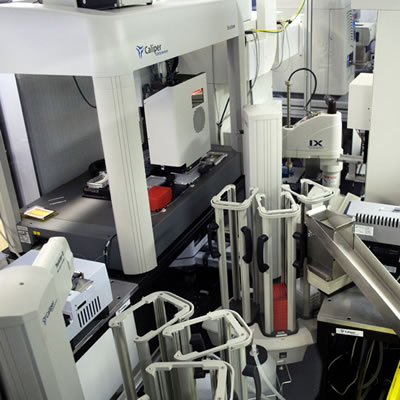
\includegraphics[width=\fwidth]{../figures/robot-scientist}
\end{frame}


\only<article>{
  Let's say we want to build a robot scientist and tell it to
  discover a cure for cancer. What does the scientist do and how can the robot replicate it??
}



\begin{frame}
  \frametitle{Drug discovery}
  \centering
  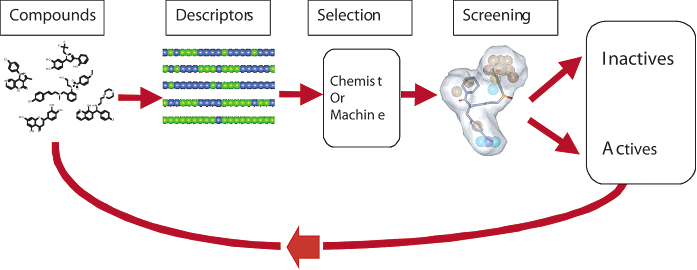
\includegraphics[width=\columnwidth]{../figures/drug-discovery-000}
\end{frame}


\only<article>{
  Simplifying the problem a bit, consider that you have a large
  number of drug candidates for cancer and you wish to discover
  those that are active against it. The ideas is that you select
  some of them, then screen them, to sort them into active and
  inactive. However, there are too many drugs to screen, so the
  process is interactive. At each cycle, we select some drugs to
  screen, classify them, and then use this information to select
  more drugs to screen. This cycle, consequently has two parts:
  1. Selecting some drugs given our current knowledge.
  2. Updating our knowledge given new evidence.
}


\begin{frame}
  \frametitle{Drawing conclusions from results}
  \begin{figure}[H]
    \centering
    \begin{tikzpicture}[line width=2pt]
      \node at (0,0) (bt) {hypothesis}; \node[select] at (0,2) (at)
      {experiment}; \node[utility] at (3,-2) (rt) {result};
      \draw[blue,->] (at) -- (rt); \node at (4,0) (bt2) {conclusion};
      \draw[red,->] (at) -- (bt2); \draw[red,->] (bt) -- (bt2);
      \draw[red,->] (rt) -- (bt2);
    \end{tikzpicture}
    \only<article>{
      \caption{Dependence diagram between selection of an experiment, formulation of a hypothesis, and drawing of a conclusion. The result depends only on the experiment. However, the conclusion depends on the experiment, hypothesis and the obtained result. The red lines indicate computational dependencies, while the blue lines indicate physical dependencies.}
    }
    \label{fig:drawing-conclusions}
  \end{figure}
\end{frame}

\only<article>{
  In general, we would like to have some method which can draw
  conclusions from results. This involves starting with a
  hypothesis, performing an experiment to verify or refute it,
  obtain some experimental result; and then concluding for or
  against the hypothesis. Here the arrows show dependencies
  between these variables. So what do we mean by "hypothesis" in this case?
}

\subsection{Bayesian inference.}
\begin{frame}
  \frametitle{Tycho Brahe's minute eye measurements}
  \begin{figure}[H]
    \centering
    \begin{columns}
      \begin{column}{0.5\textwidth}
        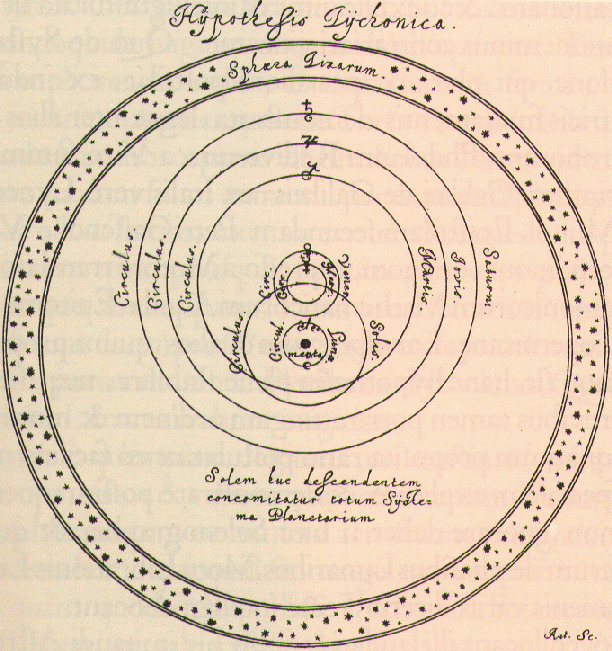
\includegraphics[width=\fwidth]{../figures/circular-orbits}
      \end{column}
      \begin{column}{0.5\textwidth}
        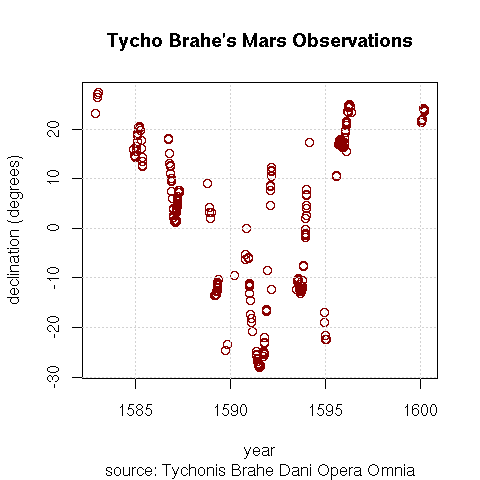
\includegraphics[width=\fwidth]{../figures/tycho-observations}
      \end{column}
    \end{columns}
    
    \caption{Tycho's measurements of the orbit of Mars and the conclusion about the actual orbits, under the assumption of an earth-centric universe with circular orbits.}
    \label{fig:tycho}
  \end{figure}
  \begin{itemize}
  \item Hypothesis: Earth-centric, Circular orbits
  \item Conclusion: \alert{Specific} circular orbits
  \end{itemize}
\end{frame}


\only<article>{
  Let's take the example of planetary orbits. Here Tycho famously
  spent 20 years experimentally measuring the location of Mars. He
  had a hypothesis: that planetary orbits were circular, but he
  didn't know which were the right orbits. When he tried to fit his data to this hypothesis, he concluded a specific circular orbit for Mars \ldots around Earth.
}


\begin{frame}
  \frametitle{Johannes Kepler's alternative hypothesis}
  \begin{columns}
    \centering
    \begin{column}{0.5\textwidth}
      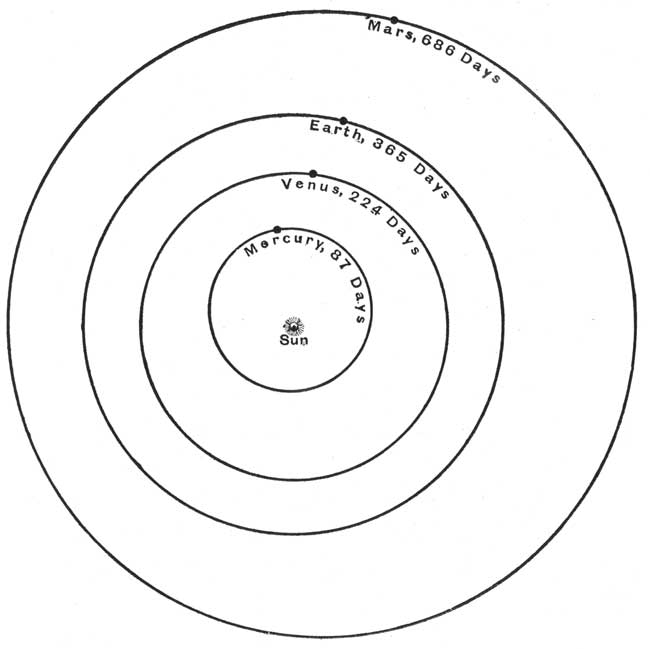
\includegraphics[width=\fwidth]{../figures/orbits}
    \end{column}
    \begin{column}{0.5\textwidth}
      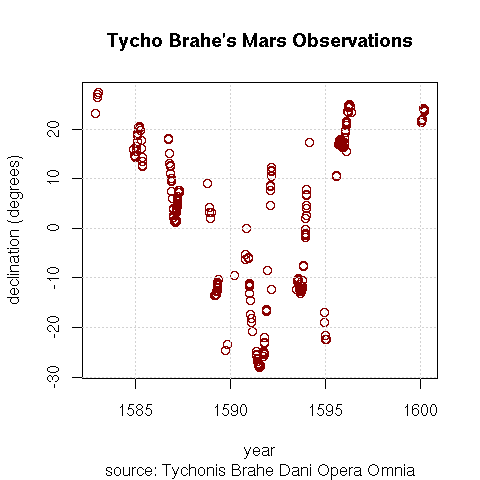
\includegraphics[width=\fwidth]{../figures/tycho-observations}
    \end{column}
  \end{columns}
  \begin{itemize}
  \item Hypothesis: Circular \alert{or} elliptic orbits
  \item Conclusion: Specific \alert{elliptic} orbits
  \end{itemize}
\end{frame}


\only<article>{
  Kepler had a more general hypothesis: that orbits could be
  circular or elliptic, and he actually accepted that the planets
  orbited the sun. This led him to the broadly correct model of all
  planets being in elliptical orbits around the sun. However, the
  actual verification that all things do not revolve around earth,
  requires different experiments.
}


\begin{frame}
  \frametitle{200 years later, Gauss formalised this statistically}
  \begin{columns}
    \begin{column}{0.5\textwidth}
      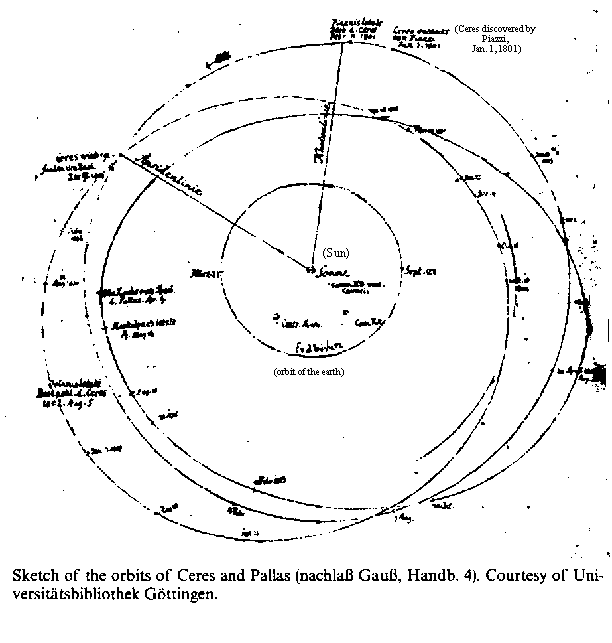
\includegraphics[width=\fwidth]{../figures/gauss-diagram}
    \end{column}
    \begin{column}{0.5\textwidth}
      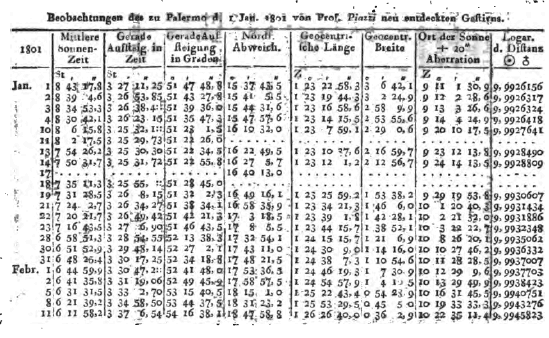
\includegraphics[width=\fwidth]{../figures/SeptemberTable}
    \end{column}
  \end{columns}
\end{frame}


\only<article>{
  Later on, Gauss collected even more experimental data to calculate the orbit of Ceres. He did this using one of the first formal statistical methods; this allowed him to avoid cheating (like Kepler did, to accentuate his finding that orbits were elliptical).
}


\begin{frame}
  \frametitle{A warning: The dead salmon mirage}
  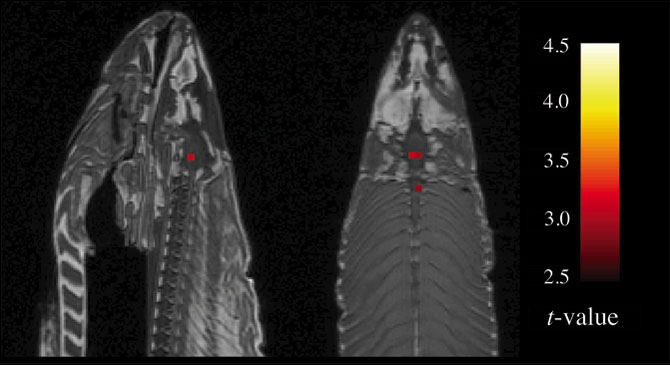
\includegraphics[width=\fwidth]{../figures/fmri-salmon}
\end{frame}


\only<article>{
  It is quite easy to draw the wrong conclusions from applying
  machine learning / statistics to your data. For example, it was
  fashionable to perform fMRI studies in humans to see whether some
  neurons have a particular functional role. There were even
  articles saying that "we found the neurons encoding for Angelina
  Jolie". So some scientists tried to replicate those results. They
  took a dead salmon, and put it an fMRI scanner. They checked its
  brain activity when it was shown images of happy or sad
  people. Perhaps surprisingly, they found an area of the brain that
  was correlated with the pictures - so it seemed, as though the
  dead salmon could distinguish photos of happy people from sad
  ones. However, this was all due to a misapplication of
  statistics. In this course, we will try and teach you to avoid
  such mistakes.

}


\begin{frame}
  \frametitle{Planning future experiments}
  \centering
  \begin{tikzpicture}[line width=2pt]
    \node at (0,0) (bt) {hypothesis};
    \node[select] at (0,2) (at) {experiment};
    \node[utility] at (3,-2) (rt) {result};
    \draw[blue,->] (at) -- (rt);
    \node at (4,0) (bt2) {conclusion};
    \draw[red,->] (at) -- (bt2);
    \draw[red,->] (bt) -- (bt2);
    \draw[red,->] (rt) -- (bt2);
  \end{tikzpicture}
\end{frame}

\only<article>{
  I mentioned before that we must decide what experiment to do. This is indeed difficult, especially in setting such as drug discovery where the number of experiments is huge.  However, conceptually, there is a simple and elegant solution to this problem.
}


\begin{frame}
  \frametitle{Planning experiments is like Tic-Tac-Toe}
  \begin{center}
    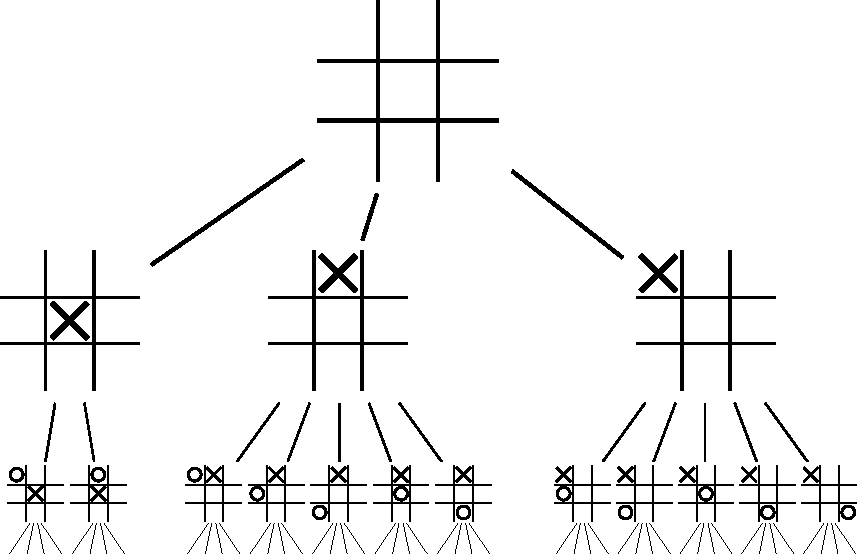
\includegraphics[width=\textwidth]{../figures/Tic-tac-toe-game-tree}
  \end{center}
\end{frame}


\only<article>{
  The basic idea is to think of experiment design as a game between the scientist and Nature. At every step, the scientist plays an X to  denote an experiment. Then Nature responds with an Observation. The main difference from a game is that Nature is (probably) not adversarial. We can also generalise this idea to problems in robotics, etc.
}

\only<presentation>{
  \begin{frame}
    \frametitle{Eve, another robot scientist}
    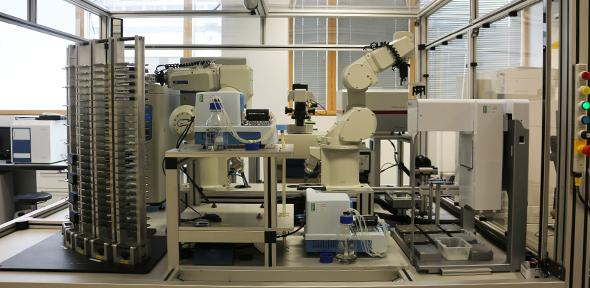
\includegraphics[width=\textwidth]{../figures/eve.jpg}
    Discovered a malaria drug
  \end{frame}
}
\only<article>{
  These kinds of techniques, coming from the reinforcement learning literature have been successfully used at the university of Manchester to create a robot, called Eve, that recently (re)-discovered a malaria drug.
}

\subsection{Course overview}

\begin{frame}
  \frametitle{Machine learning in practice}
  \begin{block}{Avoiding pitfalls}
    \begin{itemize}
    \item Choosing hypotheses.
    \item Correctly interpreting conclusions.
    \item Using a good testing methodology.
    \end{itemize}
  \end{block}
  \begin{block}{Machine learning in society}
    \begin{itemize}
    \item<alert@2> Privacy \uncover<2->{--- Credit risk.}
    \item<alert@3> Fairness \uncover<3->{--- Job market.}
    \item<alert@4> Safety \uncover<4->{--- Medicine.}
    \end{itemize}
  \end{block}
\end{frame}

\only<article>{
  One of the things we want to do in this course is teach you to
  avoid common pitfalls.

  Now I want to get into a different track. So far everything has
  been about pure research, but now machine learning is pervasive:
  Our phones, cars, watches, bathrooms, kettles are connected to the
  internet and send a continuous stream of data to companies. In
  addition, many companies and government actors use machine
  learning algorithms to make or support decisions. This creates a
  number of problems in privacy, fairness and safety.
}


\begin{frame}
  \frametitle{Technical topics}
  
  \begin{block}{Machine learning problems}
    \begin{itemize}
    \item Unsupervised learning. \only<article>{Loosely speaking, this is simply the problem of estimating some structure from data. In statistical terms, it is usually the problem of estimating some joint distribution of random variables under some model assumptions. Problems in unsupervised learning include clustering, anomaly detection, compression}.
    \item Supervised learning. \only<article>{In this setting data can be split in two groups of variables. One group that is always available, and another group that must be predicted. A special case of the problem is when we wish to estimate some function $f : \CX \to \CY$ from data. Classical problems in this setting are classification and regression.}
    \item Reinforcement learning. \only<article>{This is a very general sequential decision problem, where an agent must learn how to behave optimally in an unknown environment only by limited feedback and reinforcement. The standard setting involves the agent trying to maximise its (expected) cumulative reward over time.}
    \end{itemize}
  \end{block}

  \begin{block}{Algorithms and models}
    \begin{itemize}
    \item Bayesian inference and graphical models.
    \item Stochastic optimisation and neural networks.
    \item Backwards induction and Markov decision processes.
    \end{itemize}
  \end{block}
\end{frame}

\begin{frame}
  \frametitle{Course structure}
  \begin{block}{Module structure}
    \begin{itemize}
    \item \alert{Activity}-based, hands-on.
    \item Mini-lectures with short exercises in each class.
    \item Technical tutorials and labs in alternate week.
    \end{itemize}
  \end{block}

  \begin{block}{Two Mini-Projects}
    \begin{itemize}
    \item Simple decision problems: Credit risk.
    \item Sequential problems: Medical diagnostics and treatment.
    \end{itemize}
  \end{block}
\end{frame}

\begin{frame}
  \begin{block}{Further reading}
    \begin{itemize}
    \item \citet{bennett2012journal} describe how the usual
      uncorrected analysis of fMRI data leads to the conclusion that
      the dead salmon can reason about human images.
    \item \citet{Bennett2009ThePC} discuss how to perform analyses of medical images in a principled way. They also introduce the use of simulations in order to test how well a particular method is going to perform.
    \end{itemize}
  \end{block}
\end{frame}





%%% Local Variables: 
%%% mode: latex
%%% TeX-master: "notes.tex"
%%% End: 
